\section{Trees, Binomial random variables, independence} \label{s2} 

\ssn{Learning outcomes}
After studying this week you will be able to: 
\begin{itemize}
\item Use probability trees to calculate probabilities
\item Solve problems using the binomial distribution
\item Be able to explain and to use random variables and their expectations.
\end{itemize}
\end{n}  

\subsection{Preparation for the week} 

\ssn{Motivating problems} \label{mp2}
\begin{itemize}
    \item A production line produces components and it is assumed that each component independently has a probability $0.05$ of being faulty. Ten random samples are taken of the product; what is the probability that two or more are faulty? 
 \item A multiple choice test has ten questions, each having four possible answers. A student randomly guesses which answer is correct for every question.  What is the probability that they get an `A' by answering at least seven correctly? 
\end{itemize}
A little though should convince you that these problems are essentially the same: they are asking how likely we are to succeed $k$ times out of $n$ if each of the $n$ trials independently has probability $p$ of success. 
\end{n}


\ssn{How many `6's in three rolls?}
If I roll a D6 three times, what is the probability of three `6's? This is one outcome of the $6^3=216$ equally likely outcomes and so has probability $1/216$. 

Alternatively, we can think in stages. The probability of the first roll being `6' is $1/6$. The probability of the second roll then also being a `6' is $1/6$ and so the probability of the first two rolls being `6's is $(1/6)\times(1/6) = 1/36$. Finally, the probability of the third roll being a `6' is $1/6$ and so the probability of all three being `6's is $(1/6)^3 = 1/216$. 
We can sum this calculation up in a \emph{probability tree}: 

\tikzset{
  treenode/.style = {shape=rectangle, rounded corners,
                     draw, align=center, 
                     top color=white, bottom color=blue!30},
  root/.style     = {treenode, font=\Large, bottom color=red!30},
  env/.style      = {treenode},
  branch/.style = {treenode, bottom color=blue!10},  
  dummy/.style    = {circle,draw}
}
\tikzstyle{level 1}=[level distance=3.5cm, sibling distance=3.5cm]
\tikzstyle{level 2}=[level distance=3.5cm, sibling distance=2cm]

\begin{center}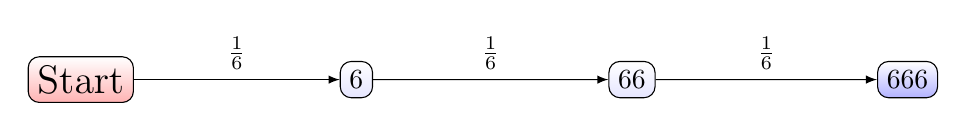
\begin{tikzpicture}
[
grow=right,
    edge from parent/.style = {draw, -latex},
    every node/.style       = {font=\normalsize}
  ]
\node[root]{Start}
child {
    node[branch]{6}
    child {
        node[branch]{66}
        child {
            node[env]{666}
            edge from parent node[above] {$\frac{1}{6}$}                      }
        edge from parent node[above] {$\frac{1}{6}$}
        }                
    edge from parent node[above] {$\frac{1}{6}$}        
    }  ;           
\end{tikzpicture}
\end{center} 
\smallskip 
You may feel this tree has fewer branches than a good tree should have. Of course, other things could happen along the way which we have omitted. All the branches appear in the full tree in Table~\ref{bigtree}, where we write `x' for a roll that is not a `6'.  

\begin{table}[h] 
\tikzstyle{level 1}=[level distance=3.5cm, sibling distance=5.0cm]
\tikzstyle{level 2}=[level distance=3.5cm, sibling distance=2.5cm]
\tikzstyle{level 3}=[level distance=3.5cm, sibling distance=1.3cm]

\begin{center} 
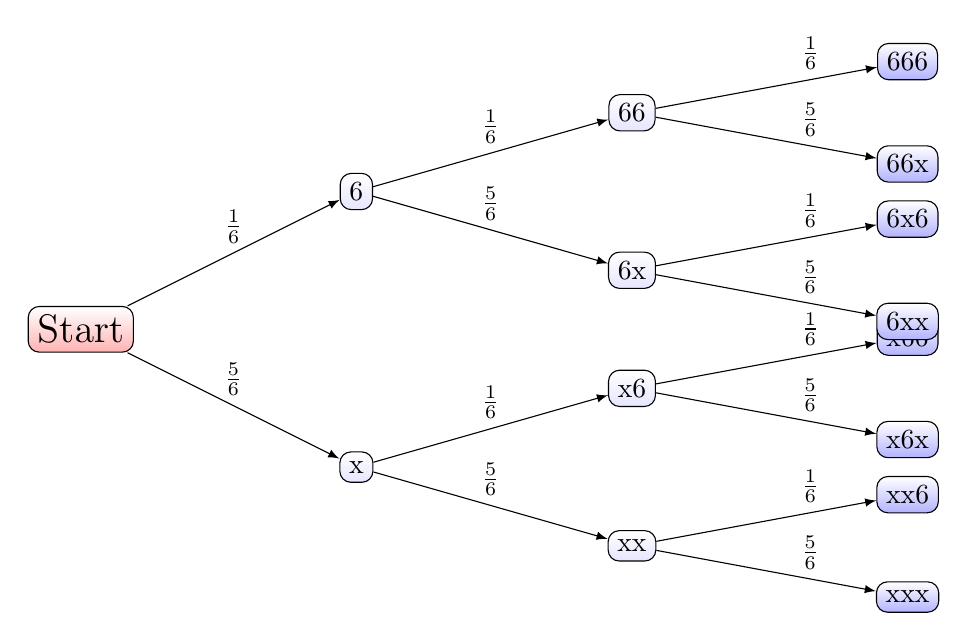
\begin{tikzpicture}
[
grow=right,
    edge from parent/.style = {draw, -latex},
    every node/.style       = {font=\normalsize}
  ]
\node[root]{Start}
child { 
    node[branch]{x}
    child { 
        node[branch]{xx}
        child{ 
             node[env]{xxx}
             edge from parent node[above,pos=0.7]{$\frac{5}{6}$}                    }
        child{ 
             node[env]{xx6}
             edge from parent node[above,pos=0.7]{$\frac{1}{6}$}      
             }               
        edge from parent node[above]{$\frac{5}{6}$} 
        }       
    child { 
        node[branch]{x6}
        child{ 
             node[env]{x6x}
             edge from parent node[above,pos=0.7]{$\frac{5}{6}$}                    }
        child{ 
             node[env]{x66}
             edge from parent node[above,pos=0.7]{$\frac{1}{6}$}      
             }               
        edge from parent node[above]{$\frac{1}{6}$} 
        }       
    edge from parent node[above]{$\frac{5}{6}$}            
    }
child { 
    node[branch]{6}
    child { 
        node[branch]{6x}
        child{ 
             node[env]{6xx}
             edge from parent node[above,pos=0.7]{$\frac{5}{6}$}                    }
        child{ 
             node[env]{6x6}
             edge from parent node[above,pos=0.7]{$\frac{1}{6}$}      
             }               
        edge from parent node[above]{$\frac{5}{6}$} 
        }       
    child { 
        node[branch]{66}
        child{ 
             node[env]{66x}
             edge from parent node[above,pos=0.7]{$\frac{5}{6}$}                    }
        child{ 
             node[env]{666}
             edge from parent node[above,pos=0.7]{$\frac{1}{6}$}      
             }               
        edge from parent node[above]{$\frac{1}{6}$} 
        }       
    edge from parent node[above]{$\frac{1}{6}$}            
    }     ;           
\end{tikzpicture} \end{center} 
\caption{Rolling a die 3 times and seeing how many `6's occur. \label{bigtree}} 
\end{table} 
\end{n}

\ssn{Using the tree}
In the tree in Table~\ref{bigtree}, the probability of an outcome is the product of the probabilities along the path leading to it.  The probability of rolling `x6x' is thus 
 \[
     \frac56 \; \frac16 \; \frac56 = \frac{25}{216}. 
 \]
 
 We could ask, for instance what is the probability of the event $A$ of getting two sixes in a row at some point in our three rolls. There are three branches of the tree with this property and adding we get 
  \[
 \PP(A) = \frac16\;\frac16 \; \frac16 + 
  \frac16\;\frac16 \; \frac56 +
    \frac56\;\frac16 \; \frac16  = \frac{11}{216}. 
  \]
Here we have used the fact that probabilities for 
disjoint events (getting two `6's in the three different ways) add. 
\end{n}

\ssn{An important example} 
What is the probability that on rolling three D6 I get exactly one `6'? 

There are exactly three routes through the tree that give this outcome and each has probability 
 \[
      \left( \frac16 \right) \left( \frac56 \right)^2 = \frac{25}{216}.
 \]
Thus the probability is 
 \[
     3 \frac{25}{216} = \frac{25}{72}. 
 \] 
\end{n}

\ssn{A generalisation}
Let us consider a general version of the problem.  Supposing we have a process that each time it is carried out produces independently a ``success'' (S) with probability $p$ or a failure (F) with probability $q=1-p$. In the examples in \S\ref{mp2}, success is finding a faulty component or correctly guessing the answer to a question.  We are assuming that each execution of the process is ``independent'', meaning that its success or failure  each time is not influenced by what might have happened before.  If we now repeat this process $n$ times, what is the probability that we get exactly $k$ successes? 
\end{n}




\ssn{Example} 
Suppose $n=10$ and $k=7$ and $p=1/4$. One particular sequence of successes and failures is $SSFFSSFSSS$. Thinking of a large probability tree, the probability of this exact sequence is 
 \[
    ppqqppqppp = p^k q^{n-k} = p^7 q^3 = \left( \frac14 \right)^7 \, \left( \frac34 \right)^3   = \frac{3^3}{4^{10}}
\]
This probability is the same for all the different sequences with seven successes. 

How many other sequences  are there with precisely seven S's?  That is the same question as asking how many ways are there of choosing seven things from ten.  It is the Binomial coefficient
 \[
       \binom{10}7 = \frac{10!}{7! \,3!} = 120. 
  \]
Adding all these possibilities, the probability of three successes in eight trials is exactly 
  \[
     \binom{10}7 p^k q^{n-k} = 120 \frac{3^3}{4^{10}} \approx 0.0031. 
  \]
\end{n}

\sse{}
Note that we have just derived the probability of getting exactly 7 out of 10 by guessing in our multiple choice quiz. Work out the probability of getting 8, 9 and 10 out of 10 and hence answer our second motivating problem. 
\end{e}

\sss
\[
    \binom{10}{7} \left( \frac13\right)^7 \left( \frac23 \right)^3 +  
    \binom{10}{8} \left( \frac13\right)^8 \left( \frac23 \right)^2 +  
    \binom{10}{9} \left( \frac13\right)^9 \left( \frac23 \right)^1 +  
    \binom{10}{10} \left( \frac13\right)^{10} \left( \frac23 \right)^0  \approx 0.019661636.
 \]
 (I give many decimal places because leaving out the 1/10 possibility only affects the fifth decimal place!) 
\end{s}


\ssn{} 
For the general problem, the probability of $k$ successes in $n$ trials is as follows.  
\tcb 
\ul{Binomial distribution} 
  \[
       \PP( \text{$k$ successes}) =  \binom nk p^k q^{n-k} =  \frac{n!}{k! \, (n-k)!} p^k q^{n-k}. 
  \]
 \etcb 
\end{n}

\ssn{Example}
I roll a D6 twelve times.  How likely is it that I roll precisely two sixes?   Here, $n=12, k=2$ and $p=1/6$. So the answer is 
 \[
    \binom{12}2 \left(\frac{1}{6}\right)^2  \left(\frac{5}{6}\right)^{10}
     \approx 0.296.
 \]
\end{n}

\sse{Exercise}
I toss a fair coin 6 times.  How likely is it that I roll $k$ heads where $k=0,1,2,3,4,5,6$? 
\end{e}
\sss 
Use the formula with $n=6$ and $p=1/2$.  For instance, $\PP(k=3) = 20/64 = 5/16$. 
\end{s}



\begin{table}[h]  
  \begin{tabular}{cc} 
    \includegraphics[width=0.45\textwidth]{images/binom15P25.png} & 
    \includegraphics[width=0.45\textwidth]{images/binom15P75.png} \\
     \includegraphics[width=0.45\textwidth]{images/binom15P5.png} & 
    \includegraphics[width=0.45\textwidth]{images/binom15P15.png} \\
  \end{tabular}
 \caption{\label{binpics} Binomial with $n=15$ and $p=0.15, 0.25, 0.5, 0.75$ in some order}
\end{table}


\sse
In table~\ref{binpics} ``probability mass functions'' for Binomial distributions with different probabilities are plotted. The height of each vertical bar is the probability of the corresponding outcome. Which is which?
\end{e}

\sss
The top row has $p=0.25$ and $p=0.75$. Note the symmetry between them. 
The bottom two are $p=0.5$ (note the symmetry about its centre) and $p=0.15$. 
\end{s}

\ssn{Another tree example} 
In Workshop~1 we calculated the win probability for Blue when rolling two six sided dice: Blue numbered $(6,3,3,3,3,3)$ versus Green numbered $(5,5,5,2,2,2)$. 

If we imagine Blue rolling first, we can draw a tree as below. 

\tikzset{
  treenode/.style = {shape=rectangle, rounded corners,
                     draw, align=center, 
                     top color=white, bottom color=blue!30},
  root/.style     = {treenode, font=\Large, bottom color=red!30},
  env/.style      = {treenode},
  branch/.style = {treenode, bottom color=blue!10},  
  dummy/.style    = {circle,draw}
}
\tikzstyle{level 1}=[level distance=3.5cm, sibling distance=3.5cm]
\tikzstyle{level 2}=[level distance=3.5cm, sibling distance=2cm]

\begin{center}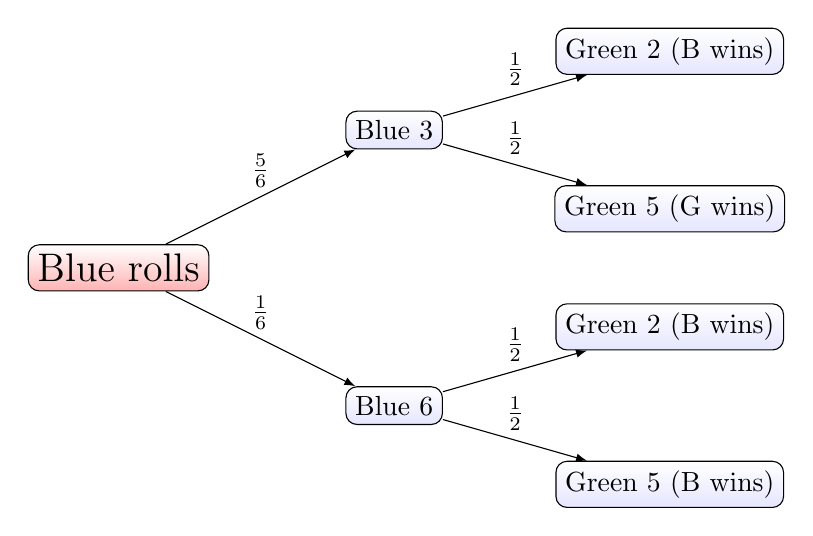
\begin{tikzpicture}
[
grow=right,
    edge from parent/.style = {draw, -latex},
    every node/.style       = {font=\normalsize}
  ]
\node[root]{Blue rolls}
child {
    node[branch]{Blue 6}
    child {
        node[branch]{Green 5 (B wins)}
        edge from parent node[above] {$\frac{1}{2}$}
        }  
    child {
        node[branch]{Green 2 (B wins)}
        edge from parent node[above] {$\frac{1}{2}$}
        }  
    edge from parent node[above] {$\frac{1}{6}$}        
    }     
child {
    node[branch]{Blue 3}
    child {
        node[branch]{Green 5 (G wins)}
        edge from parent node[above] {$\frac{1}{2}$}
        }  
    child {
        node[branch]{Green 2 (B wins)}
        edge from parent node[above] {$\frac{1}{2}$}
        }   
    edge from parent node[above] {$\frac{5}{6}$}        
    }  ;    
\end{tikzpicture}
\end{center} 
There is a single path to a Green win and that has probability $(5/6)(1/2) = 5/12$.  So blue wins with probability $1 - (5/12) = 7/12$. 

You could observe that Blue has certainly won if they roll a `6' and so one could terminate the lower branch at that point.  
\end{n} 

\sse{}
\begin{enumerate}
    \item 
Compute the `Red v Blue' and `Green v Red' probabilities with a tree.
 \item Compute the win probability of Blue versus Green where the game is to roll two blue dice versus two green dice with the higher total winning. 
\end{enumerate}
Answers to these can be found in the Workshop 1 solutions. 
\end{e}



\subsection{Notes} 

\ssn{Definition: independence} \hfill
\tcb
Two events $A,B \subseteq S$ are \ul{independent} if
 \[
   \PP(A \cap B) = \PP(A) \PP(B). 
 \]
\etcb

\noindent
The event $A \cap B$ is the intersection of the two events: it occurs precisely when both $A$ and $B$ occur. 

We say two events are ``dependent'' if they are not independent. 

We will say more about independence next week.  Two events being independent means that knowing that one has occurred does not change the probability that the other occurs.  
\end{n}

\ssn{Examples}
\begin{itemize}
    \item Roll a D6 twice. Let $A$ be the event that the first roll is a `6' and let $B$ be the event that the second roll is a `6'. Then $\PP(A) = \PP(B) = 1/6$. Then $A \cap B$ is rolling `double-6' which has probability $1/36$. So $A$ and $B$ are independent.  We were using this independence in our calculations with the probability trees above. 
    \item Roll a D6 twice. Let $A$ be the event that the sum of the rolls is $5$ and let $B$ be the event that at least one `1' appears.     Then $A=\{ (1,4), (4,1),(2,3),(3,2) \} $ and so $\PP(A) = 4/36$.   Counting we find $11$ possible rolls contain at least one `1' and so $\PP(B) = 11/36$.    The event $A \cap B = \{ (1,4), (4,1)$ and so $\PP(A \cap B) = 2/36$. Checking 
     \[
        \frac2{36} \not = \frac{4}{36} \, \frac{11}{36}
     \]
     and so $A$ and $B$ are \emph{not} independent. 
      \begin{itemize}
          \item Looking at this from another angle, if we know that the sum is 5, then there are only four possibilities and two of them contain a `1':  the probability now of there being a `1' present is $1/2$. 
      \end{itemize}
\end{itemize}
It is worth noting at this stage that the very last item above is usually expressed in the form 
 \[
  \text{The \ul{conditional probability} of $B$ given $A$ is equal to $1/2$} 
 \]
which we write with the notation 
\[
   \PP( B \st A) = \frac12 
\]
where the vertical bar is read as ``given''. 
We will take up conditional probability further next week. 
\end{n}

\ssn{Definition: Random variable}
For a binomial distribution problem, the sample space $S$ might be taken to be all the possible $2^n$ length-$n$ sequences of successes and failures. But all we are interested in is the number of successes, which is a function on the sample space taking numerical values.  Thus we make the definition:

\tcb
A \ul{random variable} is a function on the sample space.
\etcb 
We usually use capital letters from late in the alphabet (very often $X$) as the symbol for a random variable. 

In probability we will often de-emphasise or even ignore the sample space and work with the random variable directly. 

These capital $X$ random variable gadgets are a bit like the $x$ that appears for a variable in algebra, except that we imagine it takes various different values probabilistically. 

We will assume for now that our random variables, like our sample spaces, are \ul{discrete}; this means that they take a finite or countably infinite number of possible values $x_1, x_2, \dots$.  
\end{n}

\ssn{Uniform random variable}
The \emph{standard uniform random variable} on $\{1,2, \dots , n\}$ is a random variable $X$ such that 
 \[
   \PP(X=k) = \frac1n \quad \text{for $k \in \NN, \;  k \leq n$}
 \]
Rolling an $n$-sided die (which we usually denote `Dn') is assumed to be such a random variable.

We use the symbol `$\sim$' to indicate that a random variable is distributed according to a standard law. Thus here we will sometimes write 
 \[
     X \sim \mathop{Unif}(1,\dots, n). 
 \]
\end{n} 

\ssn{Bernoulli random variable}
A \emph{Bernoulli random variable} with parameter $p$ (where $0 \leq p \leq 1$) is a random variable such that $\PP(X=1) = p$ and $\PP(X=0) = q$ where $q=1-p$. 

We will write $X \sim \mathop{Bern}(p)$ to indicate that $X$ is distributed as a Bernoulli random variable with parameter $p$. 

So a Bernoulli random variable is a one-off trial that succeeds with probability $p$.  It is the trivial $n=1$ case of a binomial random variable.
\end{n}

\ssn{Binomial random variable}
A Binomial random variable with parameters $n \in \NN$ and $p$ (where $0 \leq p \leq 1$) is a random variable taking values $\{ 0,1, \dots , n \}$ with 
 \[
   \PP(X=k) =   \binom nk p^k q^{n-k} =  \frac{n!}{k! \, (n-k)!} p^k q^{n-k}
 \]
 We will write $X \sim \mathop{Binom}(n,p)$ to indicate that $X$ is distributed as a binomial random variable with parameters $n$ and $p$.
\end{n}
 
 \ssn{Events}
 When working with a random variable $X$, events can be defined in terms of the values taken.  So for instance $X=3$ and $1 \leq X \leq 4$ define events. Thus we can refer to their probabilities $\PP(X=3)$ and $\PP( 1 \geq X \leq 4)$. 
\end{n}
 
 \ssn{Definition: Independence of random variables} 
 If we have two random variables $X,Y$ defined on the same sample space we say that
 \tcb 
 $X$ and $Y$ are \ul{independent} if for all values $x,y$ we have 
 \[
     \PP( \text{$X=x$ and $Y=y$} ) \quad = \quad \PP( X=x) \, \PP(Y=y).
  \]
 \etcb 
\end{n}
 
\ssn{The idea of expected value}
Roll a 4-sided die 1000 times and add together your scores. You would expect to roll about 250 each of 1,2,3 and 4 and if you did that exactly you would score 
\[
   (250 \times 1) +  (250 \times 2) + (250 \times 3) + (250 \times 4 ) = 2500.  
\]
You could rewrite that as 
\[
  1000 \left( \left( \frac{1}{4}  \times 1\right) 
   + \left( \frac{1}{4}  \times 2\right) 
   +\left( \frac{1}{4}  \times 3\right) +\left( \frac{1}{4}  \times 4\right) \right) = 1000 \times \frac{5}{2}    
\]
and we see that each roll of the die contributes an ``expected value'' of $\frac{5}{2}$ to the total. 
\end{n}

\ssn{Definition: Expected value}
Suppose that the random variable $X$ takes a finite or countable number of different numerical values $x_i$. Let the probability that $X$ takes the value $x_i$ be denoted $p_i$ so that 
 \[
     \PP (X=x_i) = p_i \qquad \text{where} \sum_i p_i = 1. 
 \]
\tcb
The \ul{expected value} $\EE(X)$ of $X$ is defined to be 
 \[
  \EE(X)  = \sum_i p_i x_i
 \]
 where the sum is taken over all relevant values of $i$.
 \etcb
 (If there are countably infinite outcomes the sum may turn out infinite and so $\EE(X)$ may not exist.) 
\end{n}
 
\ssn{Examples}   \label{exex} 
\begin{enumerate}
\item In the 4-sided die example above the possible values of $X$ are 1,2,3,4 and so $x_1=1, x_2=2, x_3 = 3, x_4=4$. Correspondingly, $p_1=p_2=p_3=p_4 = \frac{1}{4}$. Calculating, we find that 
 \[
    \EE(X) = \frac14 \times 1 + 
       \frac14 \times 2 + 
     \frac14 \times 3 + 
     \frac14 \times 4   
    = \frac{5}{2}. 
  \]
\item I toss a coin three times and let $X$ denote the number of times that I get H.  Then from earlier, 
\[
  \PP(X=0)=\frac{1}{8}, \quad  \PP(X=1)=\frac{3}{8}, \quad  \PP(X=2)=\frac{3}{8}, \quad  \PP(X=3)=\frac{1}{8}
\]
and so 
\[
 \EE(X) = \frac{1}{8} \times 0 + \frac{3}{8} \times 1 + \frac{3}{8} \times 2 + \frac{1}{8} \times 3  = \frac{3}{2}.  
\]
\item Let $X \sim \mathop{Bern}(p)$ be a Bernoulli random variable.   Then $X$ takes the values $0,1$ with probabilities $(1-p), p$ respectively. Thus 
 \[
    \EE(X) = (1-p) 0 + p 1 = p. 
 \]
\end{enumerate}
\end{n}

\ssn{The betting metaphor}
It may help to think in terms of betting. For instance, in the last example one might imagine a game where somebody tosses three coins of equal worth and has to give you all those that come down ``heads''.  Then a ``fair'' price to pay for playing each game would be $2.5$ coins in the sense that if you played many times you would expect to come out even in the long run. 
\end{n}


 \ssn{Definition: linear combinations of random variables}
 Let $X,Y$ be random variables on the same sample space. Let $k \in \RR$. Then we can define a random variable $kX$ whose value is $k$ times whatever the value of $X$ is. 
 
 We can also consider a random variable $X + Y$. What this means is that we perform our experiment which generates a value for both $X$ and $Y$ and we take the sum to get the value of $X+Y$. 
\end{n}
 
 \ssn{Theorem: additivity of expected value}
 Let $X,Y$ be discrete random variables.  Then 
  \begin{itemize}
      \item $\EE(k X) = k \EE(X)$
      \item $\EE(X+Y) = \EE(X) + \EE(Y)$
  \end{itemize}
  \begin{proof}
The first claim is easier.  Suppose $X$ takes values $x_1,x_2,\dots$ with probabilities $p_1, p_2, \dots$.  Then $kX$ takes values $k x_1, k x_2 , \dots$ with those same probabilities.  So
 \[
   \EE(kX) = \sum_i p_i k x_i = k \sum_i p_i  x_i = k \EE(X).
 \]
 
 For the second statement, suppose $Y$ takes values $y_1, y_2, \dots$ with probabilities $q_1, q_2, \dots$.   Now, thinking in terms of events, 
  \[
      \{ X=x_i \} = \bigcup_j  \{ \text{$X = x_i$ and $Y=y_j$} \} 
  \]
  which is a disjoint union.  So taking probabilities,
 \[
    \PP(X=x_i) =  \sum_{j} \PP(\text{$X=x_i$ and $Y=y_j$}). 
 \]
 
 Now consider 
\begin{eqnarray*}
 \EE(X+Y) &=& \sum_{\text{all pairs $(i,j)$}}  \PP(\text{$X=x_i$ and $Y=j_j$}) (x_i+y_j)  \\
 &=& \sum_{i} \sum_j   \PP(\text{$X=x_i$ and $Y=x_j$}) x_i +
        \sum_{j} \sum_i   \PP(\text{$X=x_i$ and $Y=j_j$}) y_j \\
  &=&  \sum_{i}    \PP(\text{$X=x_i$}) x_i +
        \sum_{j}   \PP(\text{$Y=j_j$}) y_j \\
  &=& \EE(X) + \EE(Y).
\end{eqnarray*}
Going from the first to the second line, we are splitting $x_i + y_j$ into two terms and we are also using the fact that a sum over all combinations of values of $i$ and $j$ can be done by taking the sum over $j$ and then the sum over $i$ or \emph{vice versa}. 
 \end{proof}
 This result extends easily to sums of more random variables by e.g.\ treating $X+Y+Z$ as  $(X+Y)+Z$. 
\end{n}
 
 \ssn{Slogan} \hfill 
   \tcb 
   \begin{center} 
   {\Large Expectations of random variables add}  \\[1.5ex] 
    This is true even if they are not independent.
   \end{center}
   \etcb
\end{n}
 
 \ssn{Example} 
  Let $X$ be the random variable that is the result of rolling three D6 and taking  the sum.  Then we can write $X = X_1 + X_2 +X_3$ where $X_j$ is the number appearing on the $j$th die.  Each of the $X_j$ has expected value $7/2$. Thus 
   \[
     \EE(X) = \frac72 + \frac 72 + \frac72 = \frac{21}{2}. 
   \]
\end{n}
 
 \ssn{Proposition: Expectation of binomial random variable}
 Let $X \sim \mathop{Binom}(n,p)$.  Then $\EE(X) = np$. 
 \begin{proof} 
 We can write 
  \[
      X = X_1 + X_2 + \dots + X_n
  \]
 where $X_j$ is the Bernoulli random variable which takes the value $1$ if the $j$th trial is successful and $0$ otherwise. From \S\ref{exex} we know that $\EE(X_j) = p$ and therefore we know that $\EE(X) = np$. 
 \end{proof}
 You might argue that this result is not surprising: if we try $n$ times where each try independently succeeds with probability $p$, we might ``expect'' $np$ successes.  
\end{n}
 
 \ssp{} 
  I toss a coin $n$ times. Let $X$ be the number of consecutive pairs of H that I get. (So a sequence like $T,H,H,H,T$ would count as two such pairs.) What is the expected value of $X$? (Hint: it may help to consider random variables $X_j$ where $X_j=1$ if the $j$th and $(j+1)$th tosses are both H and $X_j=0$ otherwise.) 
  
  You should be able to check your answer be working out the probability explicitly for $n=2,3,4$. 
 \end{e}
 
 \ssp{}
 Imagine a game of tennis where there is no ``deuce / advantage'' and the first player to four points wins.  Suppose player A wins each point independently with probability $p$ and $B$ wins with probability $q=1-p$.  How likely is player A to win? (Hint: imagine that instead of stopping when one player reaches four points, the players play 7 points and then stop. At that point, one but not both players must have scored 4 points.)  It is not easy to simplify the answer but you could ask Wolfram Alpha to, or you could plot the answer against $p$. 
 \end{e}
 
 \ssp{} 
 You and I play the following game. Hidden from you, I put a coin in my hand: with probability $p$ it is a 10 pence coin and otherwise it is a 20 pence coin. 
 You now guess which coin is in my hand: you guess it is 20 pence with probability $q$ and otherwise you guess it is a 10 pence coin.  You win the coin if you guess correctly and otherwise win nothing.  What is your expected gain in pence from playing this game once with me? 
 
 Challenge: suppose we are going to play repeatedly and you want to maximise your gain and I wish to minimise my loss. What value of $p$ should I choose and what value of $q$ should you choose? (This question is somewhat ill-defined, but it does have an interesting possible answer!) 
 \end{e}